
%% bare_conf_compsoc.tex
%% V1.4b
%% 2015/08/26
%% by Michael Shell
%% See:
%% http://www.michaelshell.org/
%% for current contact information.
%%
%% This is a skeleton file demonstrating the use of IEEEtran.cls
%% (requires IEEEtran.cls version 1.8b or later) with an IEEE Computer
%% Society conference paper.
%%
%% Support sites:
%% http://www.michaelshell.org/tex/ieeetran/
%% http://www.ctan.org/pkg/ieeetran
%% and
%% http://www.ieee.org/

%%*************************************************************************
%% Legal Notice:
%% This code is offered as-is without any warranty either expressed or
%% implied; without even the implied warranty of MERCHANTABILITY or
%% FITNESS FOR A PARTICULAR PURPOSE! 
%% User assumes all risk.
%% In no event shall the IEEE or any contributor to this code be liable for
%% any damages or losses, including, but not limited to, incidental,
%% consequential, or any other damages, resulting from the use or misuse
%% of any information contained here.
%%
%% All comments are the opinions of their respective authors and are not
%% necessarily endorsed by the IEEE.
%%
%% This work is distributed under the LaTeX Project Public License (LPPL)
%% ( http://www.latex-project.org/ ) version 1.3, and may be freely used,
%% distributed and modified. A copy of the LPPL, version 1.3, is included
%% in the base LaTeX documentation of all distributions of LaTeX released
%% 2003/12/01 or later.
%% Retain all contribution notices and credits.
%% ** Modified files should be clearly indicated as such, including  **
%% ** renaming them and changing author support contact information. **
%%*************************************************************************


% *** Authors should verify (and, if needed, correct) their LaTeX system  ***
% *** with the testflow diagnostic prior to trusting their LaTeX platform ***
% *** with production work. The IEEE's font choices and paper sizes can   ***
% *** trigger bugs that do not appear when using other class files.       ***                          ***
% The testflow support page is at:
% http://www.michaelshell.org/tex/testflow/



\documentclass[conference,compsoc]{IEEEtran}
% Some/most Computer Society conferences require the compsoc mode option,
% but others may want the standard conference format.
%
% If IEEEtran.cls has not been installed into the LaTeX system files,
% manually specify the path to it like:
% \documentclass[conference,compsoc]{../sty/IEEEtran}





% Some very useful LaTeX packages include:
% (uncomment the ones you want to load)


\usepackage{listings}
\usepackage{xcolor}
\lstset{
  showstringspaces=false,
  commentstyle=\color{red},
  keywordstyle=\color{blue}
}

% *** MISC UTILITY PACKAGES ***
%
%\usepackage{ifpdf}
% Heiko Oberdiek's ifpdf.sty is very useful if you need conditional
% compilation based on whether the output is pdf or dvi.
% usage:
% \ifpdf
%   % pdf code
% \else
%   % dvi code
% \fi
% The latest version of ifpdf.sty can be obtained from:
% http://www.ctan.org/pkg/ifpdf
% Also, note that IEEEtran.cls V1.7 and later provides a builtin
% \ifCLASSINFOpdf conditional that works the same way.
% When switching from latex to pdflatex and vice-versa, the compiler may
% have to be run twice to clear warning/error messages.






% *** CITATION PACKAGES ***
%
\ifCLASSOPTIONcompsoc
  % IEEE Computer Society needs nocompress option
  % requires cite.sty v4.0 or later (November 2003)
  \usepackage[nocompress]{cite}
\else
  % normal IEEE
  \usepackage{cite}
\fi
% cite.sty was written by Donald Arseneau
% V1.6 and later of IEEEtran pre-defines the format of the cite.sty package
% \cite{} output to follow that of the IEEE. Loading the cite package will
% result in citation numbers being automatically sorted and properly
% "compressed/ranged". e.g., [1], [9], [2], [7], [5], [6] without using
% cite.sty will become [1], [2], [5]--[7], [9] using cite.sty. cite.sty's
% \cite will automatically add leading space, if needed. Use cite.sty's
% noadjust option (cite.sty V3.8 and later) if you want to turn this off
% such as if a citation ever needs to be enclosed in parenthesis.
% cite.sty is already installed on most LaTeX systems. Be sure and use
% version 5.0 (2009-03-20) and later if using hyperref.sty.
% The latest version can be obtained at:
% http://www.ctan.org/pkg/cite
% The documentation is contained in the cite.sty file itself.
%
% Note that some packages require special options to format as the Computer
% Society requires. In particular, Computer Society  papers do not use
% compressed citation ranges as is done in typical IEEE papers
% (e.g., [1]-[4]). Instead, they list every citation separately in order
% (e.g., [1], [2], [3], [4]). To get the latter we need to load the cite
% package with the nocompress option which is supported by cite.sty v4.0
% and later.





% *** GRAPHICS RELATED PACKAGES ***
%
\ifCLASSINFOpdf
   \usepackage[pdftex]{graphicx}
%   declare the path(s) where your graphic files are
%   \graphicspath{{../img/}{../jpeg/}}
%   and their extensions so you won't have to specify these with
%   every instance of \includegraphics
%   \DeclareGraphicsExtensions{.pdf,.jpeg,.png}
\else
  % or other class option (dvipsone, dvipdf, if not using dvips). graphicx
  % will default to the driver specified in the system graphics.cfg if no
  % driver is specified.
  % \usepackage[dvips]{graphicx}
  % declare the path(s) where your graphic files are
  % \graphicspath{{../eps/}}
  % and their extensions so you won't have to specify these with
  % every instance of \includegraphics
  % \DeclareGraphicsExtensions{.eps}
\fi
% graphicx was written by David Carlisle and Sebastian Rahtz. It is
% required if you want graphics, photos, etc. graphicx.sty is already
% installed on most LaTeX systems. The latest version and documentation
% can be obtained at: 
% http://www.ctan.org/pkg/graphicx
% Another good source of documentation is "Using Imported Graphics in
% LaTeX2e" by Keith Reckdahl which can be found at:
% http://www.ctan.org/pkg/epslatex
%
% latex, and pdflatex in dvi mode, support graphics in encapsulated
% postscript (.eps) format. pdflatex in pdf mode supports graphics
% in .pdf, .jpeg, .png and .mps (metapost) formats. Users should ensure
% that all non-photo figures use a vector format (.eps, .pdf, .mps) and
% not a bitmapped formats (.jpeg, .png). The IEEE frowns on bitmapped formats
% which can result in "jaggedy"/blurry rendering of lines and letters as
% well as large increases in file sizes.
%
% You can find documentation about the pdfTeX application at:
% http://www.tug.org/applications/pdftex





% *** MATH PACKAGES ***
%
%\usepackage{amsmath}
% A popular package from the American Mathematical Society that provides
% many useful and powerful commands for dealing with mathematics.
%
% Note that the amsmath package sets \interdisplaylinepenalty to 10000
% thus preventing page breaks from occurring within multiline equations. Use:
%\interdisplaylinepenalty=2500
% after loading amsmath to restore such page breaks as IEEEtran.cls normally
% does. amsmath.sty is already installed on most LaTeX systems. The latest
% version and documentation can be obtained at:
% http://www.ctan.org/pkg/amsmath





% *** SPECIALIZED LIST PACKAGES ***
%
%\usepackage{algorithmic}
% algorithmic.sty was written by Peter Williams and Rogerio Brito.
% This package provides an algorithmic environment fo describing algorithms.
% You can use the algorithmic environment in-text or within a figure
% environment to provide for a floating algorithm. Do NOT use the algorithm
% floating environment provided by algorithm.sty (by the same authors) or
% algorithm2e.sty (by Christophe Fiorio) as the IEEE does not use dedicated
% algorithm float types and packages that provide these will not provide
% correct IEEE style captions. The latest version and documentation of
% algorithmic.sty can be obtained at:
% http://www.ctan.org/pkg/algorithms
% Also of interest may be the (relatively newer and more customizable)
% algorithmicx.sty package by Szasz Janos:
% http://www.ctan.org/pkg/algorithmicx




% *** ALIGNMENT PACKAGES ***
%
%\usepackage{array}
% Frank Mittelbach's and David Carlisle's array.sty patches and improves
% the standard LaTeX2e array and tabular environments to provide better
% appearance and additional user controls. As the default LaTeX2e table
% generation code is lacking to the point of almost being broken with
% respect to the quality of the end results, all users are strongly
% advised to use an enhanced (at the very least that provided by array.sty)
% set of table tools. array.sty is already installed on most systems. The
% latest version and documentation can be obtained at:
% http://www.ctan.org/pkg/array


% IEEEtran contains the IEEEeqnarray family of commands that can be used to
% generate multiline equations as well as matrices, tables, etc., of high
% quality.




% *** SUBFIGURE PACKAGES ***
%\ifCLASSOPTIONcompsoc
%  \usepackage[caption=false,font=footnotesize,labelfont=sf,textfont=sf]{subfig}
%\else
%  \usepackage[caption=false,font=footnotesize]{subfig}
%\fi
% subfig.sty, written by Steven Douglas Cochran, is the modern replacement
% for subfigure.sty, the latter of which is no longer maintained and is
% incompatible with some LaTeX packages including fixltx2e. However,
% subfig.sty requires and automatically loads Axel Sommerfeldt's caption.sty
% which will override IEEEtran.cls' handling of captions and this will result
% in non-IEEE style figure/table captions. To prevent this problem, be sure
% and invoke subfig.sty's "caption=false" package option (available since
% subfig.sty version 1.3, 2005/06/28) as this is will preserve IEEEtran.cls
% handling of captions.
% Note that the Computer Society format requires a sans serif font rather
% than the serif font used in traditional IEEE formatting and thus the need
% to invoke different subfig.sty package options depending on whether
% compsoc mode has been enabled.
%
% The latest version and documentation of subfig.sty can be obtained at:
% http://www.ctan.org/pkg/subfig




% *** FLOAT PACKAGES ***
%
%\usepackage{fixltx2e}
% fixltx2e, the successor to the earlier fix2col.sty, was written by
% Frank Mittelbach and David Carlisle. This package corrects a few problems
% in the LaTeX2e kernel, the most notable of which is that in current
% LaTeX2e releases, the ordering of single and double column floats is not
% guaranteed to be preserved. Thus, an unpatched LaTeX2e can allow a
% single column figure to be placed prior to an earlier double column
% figure.
% Be aware that LaTeX2e kernels dated 2015 and later have fixltx2e.sty's
% corrections already built into the system in which case a warning will
% be issued if an attempt is made to load fixltx2e.sty as it is no longer
% needed.
% The latest version and documentation can be found at:
% http://www.ctan.org/pkg/fixltx2e


%\usepackage{stfloats}
% stfloats.sty was written by Sigitas Tolusis. This package gives LaTeX2e
% the ability to do double column floats at the bottom of the page as well
% as the top. (e.g., "\begin{figure*}[!b]" is not normally possible in
% LaTeX2e). It also provides a command:
%\fnbelowfloat
% to enable the placement of footnotes below bottom floats (the standard
% LaTeX2e kernel puts them above bottom floats). This is an invasive package
% which rewrites many portions of the LaTeX2e float routines. It may not work
% with other packages that modify the LaTeX2e float routines. The latest
% version and documentation can be obtained at:
% http://www.ctan.org/pkg/stfloats
% Do not use the stfloats baselinefloat ability as the IEEE does not allow
% \baselineskip to stretch. Authors submitting work to the IEEE should note
% that the IEEE rarely uses double column equations and that authors should try
% to avoid such use. Do not be tempted to use the cuted.sty or midfloat.sty
% packages (also by Sigitas Tolusis) as the IEEE does not format its papers in
% such ways.
% Do not attempt to use stfloats with fixltx2e as they are incompatible.
% Instead, use Morten Hogholm'a dblfloatfix which combines the features
% of both fixltx2e and stfloats:
%
% \usepackage{dblfloatfix}
% The latest version can be found at:
% http://www.ctan.org/pkg/dblfloatfix




% *** PDF, URL AND HYPERLINK PACKAGES ***
%
%\usepackage{url}
% url.sty was written by Donald Arseneau. It provides better support for
% handling and breaking URLs. url.sty is already installed on most LaTeX
% systems. The latest version and documentation can be obtained at:
% http://www.ctan.org/pkg/url
% Basically, \url{my_url_here}.




% *** Do not adjust lengths that control margins, column widths, etc. ***
% *** Do not use packages that alter fonts (such as pslatex).         ***
% There should be no need to do such things with IEEEtran.cls V1.6 and later.
% (Unless specifically asked to do so by the journal or conference you plan
% to submit to, of course. )


% correct bad hyphenation here
\hyphenation{op-tical net-works semi-conduc-tor}


\begin{document}
%
% paper title
% Titles are generally capitalized except for words such as a, an, and, as,
% at, but, by, for, in, nor, of, on, or, the, to and up, which are usually
% not capitalized unless they are the first or last word of the title.
% Linebreaks \\ can be used within to get better formatting as desired.
% Do not put math or special symbols in the title.
\title{Cognitive WI-FI: A small step towards online self-learning data rate control}


% author names and affiliations
% use a multiple column layout for up to three different
% affiliations
\author{\IEEEauthorblockN{Jetse Brouwer}
\IEEEauthorblockA{Delft university of technology\\Embedded Systems\\
Mekelweg 4, 2628 CD Delft\\
Email: j.brouwer-3@student.tudelft.nl}
\and
\IEEEauthorblockN{Niels Hokke}
\IEEEauthorblockA{Delft university of technology\\Embedded Systems\\
Mekelweg 4, 2628 CD Delft\\
Email: n.h.hokke@student.tudelft.nl}
}

% conference papers do not typically use \thanks and this command
% is locked out in conference mode. If really needed, such as for
% the acknowledgment of grants, issue a \IEEEoverridecommandlockouts
% after \documentclass

% for over three affiliations, or if they all won't fit within the width
% of the page (and note that there is less available width in this regard for
% compsoc conferences compared to traditional conferences), use this
% alternative format:
% 
%\author{\IEEEauthorblockN{Michael Shell\IEEEauthorrefmark{1},
%Homer Simpson\IEEEauthorrefmark{2},
%James Kirk\IEEEauthorrefmark{3}, 
%Montgomery Scott\IEEEauthorrefmark{3} and
%Eldon Tyrell\IEEEauthorrefmark{4}}
%\IEEEauthorblockA{\IEEEauthorrefmark{1}School of Electrical and Computer Engineering\\
%Georgia Institute of Technology,
%Atlanta, Georgia 30332--0250\\ Email: see http://www.michaelshell.org/contact.html}
%\IEEEauthorblockA{\IEEEauthorrefmark{2}Twentieth Century Fox, Springfield, USA\\
%Email: homer@thesimpsons.com}
%\IEEEauthorblockA{\IEEEauthorrefmark{3}Starfleet Academy, San Francisco, California 96678-2391\\
%Telephone: (800) 555--1212, Fax: (888) 555--1212}
%\IEEEauthorblockA{\IEEEauthorrefmark{4}Tyrell Inc., 123 Replicant Street, Los Angeles, California 90210--4321}}




% use for special paper notices
%\IEEEspecialpapernotice{(Invited Paper)}




% make the title area
\maketitle

% As a general rule, do not put math, special symbols or citations
% in the abstract
\begin{abstract}

\end{abstract}

% no keywords

% For peer review papers, you can put extra information on the cover
% page as needed:
% \ifCLASSOPTIONpeerreview
% \begin{center} \bfseries EDICS Category: 3-BBND \end{center}
% \fi
%
% For peerreview papers, this IEEEtran command inserts a page break and
% creates the second title. It will be ignored for other modes.
\IEEEpeerreviewmaketitle

\section{Introduction} 
With the use of higher modulation and coding schemes (MCS) higher data rates can be achieved. however, a higher MCS also results in a higher susceptibility for noise. To maintain high data rates while ensuring connectivity a trade of has to be made between speed and availability. While algorithms do exist, they are mainly static. Our goal is to create a self-learning algorithm that dynamically learns from its environment without downtime. The algorithm is designed and tested by using the “802.11 Dynamic Rate Control Simulation” example from the MatLab WLAN toolbox  

\section{Method}
The algorithm exploits the correlation between the probability of successfully decoding a packet at a given MCS and the signal-to-noise ratio (SNR). When lowering SNR the probability for successfully decoding a package at a given MCS reduces significantly. The aim of our algorithm is to learn about this correlation and use this to it’s advantages. If the algorithm, for every possible SNR, would know the best suitable MCS it would be able to always perform at its maximum performance. Since the correlation does not necessarily has to be linear, and might change depending on channel configuration a single pre-defined correlation will not work.
To know which MCS would be the best suited for the given SNR the resulting bandwidth of the data transfer needs to be stored for later references. Besides storing the previous results it should also explore other, possibly better values for a given MCS.

\subsection{Data structure}
To use the correlation to our advantage, the data aggregated from previous measurements needs to be stored. This is be done by using a two-dimensional array, the 'LearnedValues' array. The first dimension corresponds to the SNR value. The SNR is divided in to bands where every x dB’s are grouped together to a single index. This is calculated using the formula $ index = \left \lfloor{}\frac{SNR}{x}  \right \rfloor$. The second dimension corresponds to one of the ten available MCS indices. A single element from the array then represents the data rates that can be achieved for that specific MCS and SNR combination.

If a package is decoded successfully or not is not constant, but a probability based on the SNR and MCS. Therefore when a new value is detected it should not directly overwrite the old value but create a combination of both the old and current data rate. How fast the algorithm should adopt this new value is set with the variable 'adoption rate'. This variable is a value between 1 and 0 and corresponds to the portion of the current value in the new value. The new value is given by our value-adoption formula: $Rate_{new} = Rate_{old} \times(1-adaption rate) + Rate_{current} \times adaption rate $

\subsection{Learning the data rates}
Based on the data rates the algorithm has learned, it can pick for a given SNR the best suitable MCS. It does so by first using the SNR from the previous packet as a starting point. From here it will look in the array at the column that matches that SNR range. It will look up the maximum know data rate it has seen, and use this as a possible candidate for the MCS. While history seems to be repeating, it does not always gives enough insight to act on in the future. Therefor the algorithm should also explore other values besides the best know value. Therefore the algorithm uses the variable 'LearningRate', which has a value betweeon 1 and 0, and is the probability of trying out a new MCS. The value of this MCS is chosen by the current ideal MCS plus 1, the result from this exploration will be stored in the 'LearnedValues' array. With this method the algorithm is always looking for better options.

If one of the known values becomes less suitable for some reason, this will be reflected in the 'LearnedValues' array. Based on the adoption rate it may take one or more failed packets to not be the maximum data-rate for the given MCS SNR combination anymore. 

\subsection{offline vs online learning}
Based on how many packets are being send and the learning rate, the speed by which the algorithm learns can vary greatly. However with Wi-Fi supporting up to 3000 packets per second \cite{3kPackets} it is expected that the algorithm will quickly adjust. One of the decisions that has to be made is the value of the learning rate, a high learning rate will result in a quickly adjusting system. However, when the system is reaching it's maximum it will still try to increase the MCS proportional to the learning rate. If the learning rate is set to 10\% and is at it's maximum, up to 10\% of the packets will be lost and therefore reduce the throughput

To speedup the learning process of the algorithm an offline training mechanism is implemented. This ignores the current maximum value and sends out as much packets as possible spread out over all possible MCS to gain knowledge about the correlation between the current SNR and MCS. In the simulation this is implemented by running the 100 packet long pattern for all 10 indices, 10 times each, resulting in 10000 packets to be send.

\section{Results}
After performing an offline learning run with an adoption rate of $\frac{1}{3}$ and a bin size of 1 dB we reached an overall data rate of 26.0572 mpbs. this is an 25\% improvement over the 23.295Mbps of the original.
To measure the performance of the online learning algorithm multiple consecutive runs have been done. The chosen learning rates for the test were 1\%, 5\% and 10\%. To have a fair start they all started with a run without having learned anything, from there on the algorithm was free to learn as it desired.

From picture \ref{fig:linegraph} it can be seen that the 10\% indeed learns the fastest, but also is very unstable as it is very aggressive with trying out new values. With 5\% the algorithm learns a bit slower, but still reaches the peak quiet fast. Compared to the other the 1\% learning rate learns significantly slower. Over time all three settings seem to converge to the same value. As it only took 20 runs to reach the same value as the others, but is more stable it seems to be a better value when it comes to user experience.

\begin{figure}[h!]
    \centering
    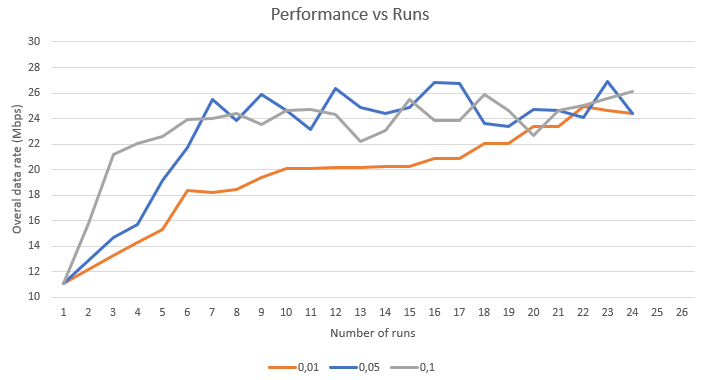
\includegraphics[width=0.5\textwidth]{img/PerformanceVSruns.PNG} 
    \caption{Performance over runs (100 packets per run) for different learning rates}
    \label{fig:linegraph}
\end{figure}


\section{Conclusion and further work}
With an overall data rate of 26 mpbs the dynamic algorithm described in the paper shows an improvement of 25\% over the original one. As the algorithm is self learning it will be able to adapt to its environment.  

As the system begins with the lowest MCS the chance of finding an better MCS is way higher at the start of the run than at the end. Later in the run the chance of finding a to high MCS which results in a failed package becomes larger and larger. The current learning rate is a static number, every x samples a new MCS is tested. It would be better to start with a high learning rate and slowly reduce it further in the run. An dynamic learning rate could result in faster learning while reducing the number of failures due to high MCS values. further research can be done on how to dynamically change this learning rate for the optimal result. 


% conference papers do not normally have an appendix


% use section* for acknowledgment

% trigger a \newpage just before the given reference
% number - used to balance the columns on the last page
% adjust value as needed - may need to be readjusted if
% the document is modified later
%\IEEEtriggeratref{8}
% The "triggered" command can be changed if desired:
%\IEEEtriggercmd{\enlargethispage{-5in}}

% references section

% can use a bibliography generated by BibTeX as a .bbl file
% BibTeX documentation can be easily obtained at:
% http://mirror.ctan.org/biblio/bibtex/contrib/doc/
% The IEEEtran BibTeX style support page is at:
% http://www.michaelshell.org/tex/ieeetran/bibtex/
%\bibliographystyle{IEEEtran}
% argument is your BibTeX string definitions and bibliography database(s)
%\bibliography{IEEEabrv,../bib/paper}
%
% <OR> manually copy in the resultant .bbl file
% set second argument of \begin to the number of references
% (used to reserve space for the reference number labels box)
\begin{thebibliography}{1}

\bibitem{3kPackets}
Pengyu Zhang, \emph{Enabling Practical Backscatter Communication for On-body Sensors}, SIGCOMM ’16, August 22-26, 2016, Florianopolis , Brazil 

\end{thebibliography}



% that's all folks
\end{document}


